\documentclass[9pt,twocolumn,twoside]{../../styles/osajnl}
\usepackage{fancyvrb}
\journal{i524} 
\usepackage{titlesec}
\usepackage{etoolbox}
\usepackage[section]{placeins}

\makeatletter
\patchcmd{\ttlh@hang}{\parindent\z@}{\parindent\z@\leavevmode}{}{}
\patchcmd{\ttlh@hang}{\noindent}{}{}{}
\makeatother



\title{Deployment and performance analysis of a Storm cluster on various cloud environments}

\author[1,*]{Vasanth Methkupalli}
\author[1,**]{Ajit Balaga}


\affil[1]{School of Informatics and Computing, Bloomington, IN 47408, U.S.A.}

\affil[*]{Corresponding authors: mvasanthiiit@gmail.com}
\affil[**]{Corresponding authors: ajit.balaga@gmail.com}


\dates{Project-P015, \today}

\ociscodes{Storm, Ansible, Java, Python}

% replace this with your url in github/gitlab
\doi{Report: \url{https://github.com/cloudmesh/classes/blob/master/project/S17-IR-P015/report/report.pdf}\\
Code: \url{https://github.com/cloudmesh/cloudmesh.storm}}


\begin{abstract}
Apache Storm is a free and open source distributed realtime
computation system. Storm makes it easy to reliably process unbounded
streams of data, doing for realtime processing what Hadoop did for
batch processing. Storm is simple, can be used with any programming
language. Storm has many use cases: realtime analytics, online machine
learning, continuous computation, distributed RPC etc. Storm is really
fast at data processing: a sample benchmark clocked it at over a
million tuples processed per second per node. It is scalable,
fault-tolerant, guarantees that data will be processed, and is easy to
set up and operate. Storm integrates with the queueing and database
technologies we already use. Storm is currently being used to run
various critical computations in Twitter at scale, and in real-time,
this led us to explore and deploy it on various cloud. In this paper
we try to deploy storm on various clouds and benchmark the performance
on various data, doing real time processing on sample datasets. First,
we describe the architecture of Storm, its deployment and its methods
for distributed scaleout and fault-tolerance. We intend to perform a
deployment and performance benchmarking to realise the storm on
various clouds. We wish to identify and examine the best clouds for
storm in terms of deployment and performance.
\end{abstract}

\setboolean{displaycopyright}{true}

\begin{document}

\maketitle

%\tableofcontents

\maketitle

\section{Introduction}
Currently modern data processing environments require processing
complex computation on streaming data in real-time. Places like
Twitter where each interaction with a user requires making a number of
complex decisions, often based on data that has just been created,
this mandates for a real time data processing system, Storm currently
delivers on this account and provides many other services which we
will see in the coming sections. Storm is designed to be, some of
these things we observed while running our sample projects for
deployment:

\begin{description}
\item Scalable : Nodes may be easily added or removed
  from the Storm cluster without disrupting existing data flows
  through Storm topologies see Fig 3.
\item Resilient : Fault -tolerance is crucial to Storm as it is often
  deployed on large clusters, and hardware components can fail.  The
  Storm cluster must continue processing existing topologies with a
  minimal performance impact.
\item Extensible : Storm topologies may call arbitrary external
  functions (e.g. looking up a MySQL service for the social graph),
  \cite{bronson2013tao} and thus needs a framework that allows
  extensibility.
\item  Efficient : Since Storm is used in
  real-time applications, it must have good performance
  characteristics. Storm uses a number of techniques, including
  keeping all its storage and computational data structures in memory.
\item Easy to Administer : A critical part of storm features or
  development is that it should be easy to administer. Given that
  there a lot of computations going on at every stage, tools should be
  developed which warn the user and development team of any major
  conflicts arising.
\end{description}

\section{Data Model and Architecture}
Storm data processing architecture consists of streams of tuples
flowing through topologies \cite{storm} . A topology is a directed
graph where the vertices represent computation and the edges represent
the data flow between the computation components. Vertices are further
divided into two disjoint sets, spouts and bolts. Spouts are tuple
sources for the topology.  Typical spouts pull data from queues, such
as Kafka \cite{kafka} or Kestrel. On the other hand, bolts process the
incoming tuples and pass them to the next set of bolts downstream.
Note that a Storm topology can have cycles. From the database systems
perspective, one can think of a topology as a directed graph of
operators.

\begin{figure}
  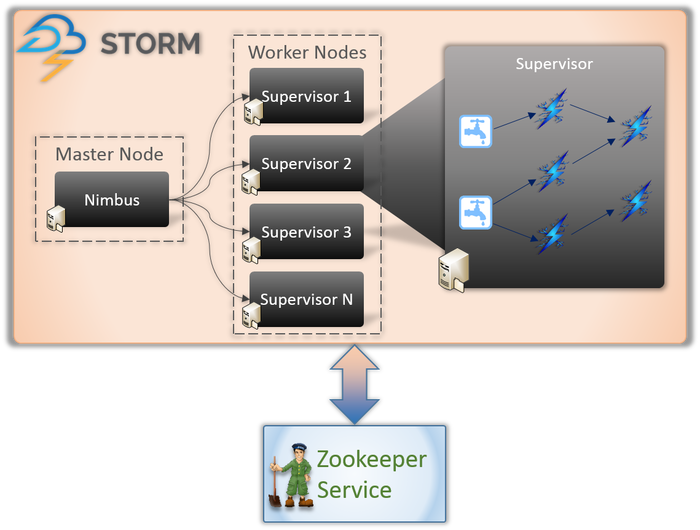
\includegraphics[width=8cm,height=8cm,keepaspectratio,width=\linewidth]{images/apache-storm.png}
  \caption{Storm Architecture}
  \label{Storm Architecture}
\end{figure}

\subsection{Storm Overview}
Storm runs on a distributed cluster. Clients submit topologies to a
master node, called the Nimbus. The nimbus is responsible for
distributing and coordinating the execution of the topology. The
actual work is done on worker nodes. Each worker node runs one or more
worker processes. At any point in time, a single machine may have more
than one worker processes, but each worker process is mapped to a
single topology see Fig \ref{Storm Architecture}. Note more than one
worker process on the same machine may be executing different part of
the same topology. Each worker process runs a JVM, in which it runs
one or more executors.  Executors are made of one or more tasks. The
actual work for a bolt or a spout is done in the task. Thus, tasks
provide intrabolt or intraspout parallelism, and the executors provide
intratopology parallelism. Worker processes serve as containers on the
host machines to run Storm topologies. Note that associated with each
spout or bolt is a set of tasks running in a set of executors across
machines in a cluster. Data is shuffled from a producer spout or bolt
to a consumer bolt (both producer and consumer may have multiple
tasks). This shuffling is like the exchange op erator in parallel
databases.

Storm supports the following types of partitioning strategies \cite{storm}:
\begin{description}  
\item Shuffle grouping, which randomly partitions the tuples.
\item Fields grouping, which hashes on a subset of the tuple
  attributes or fields.
\item All grouping, which replicates the entire stream to all the
  consumer tasks.
\item Global grouping, which sends the entire stream to a single bolt.
\item Local grouping, which sends tuples to the consumer bolts in the
  same executor.
\end{description}

The partitioning strategy is extensible and a topology can define and
use its own partitioning strategy.  Each worker node runs a Supervisor
that communicates with Nimbus.  The cluster state is maintained in
Zookeeper \cite{www-zookeeper}, and Nimbus is responsible for scheduling
the topologies on the worker nodes and monitoring the progress of the
tuples flowing through the topology. Loosely, a topology can be
considered as a logical query plan from a database systems
perspective. As a part of the topology, the programmer specifies how
many instances of each spout and bolt must be spawned. Storm creates
these instances and also creates the interconnections for the data
flow. We note that currently, the programmer has to specify the number
of instances for each spout and bolt. Part of future work is to
automatically pick and dynamically changes this number based on some
higher-level objective, such as a target performance objective.

\subsubsection{Storm Internal Architecture}
In this section, we describe the key components of Storm), and how
these components interact with each other.

\subsubsection{Nimbus and Zookeeper}
Nimbus plays a similar role as the “JobTracker” in Hadoop, and is the
touchpoint between the user and the Storm system. Nimbus is an Apache
Thrift service and Storm topology definitions are Thrift objects.  To
submit a job to the Storm cluster (i.e. to Nimbus), the user describes
the topology as a Thrift object and sends that object to Nimbus. With
this design, any programming language can be used to create a Storm
topology.

As part of submitting the topology, the user also uploads the user
code as a JAR file to Nimbus. Nimbus uses a combination of the local
disk(s) and Zookeeper to store state about the topology. Currently the
user code is stored on the local disk(s) of the Nimbus machine, and
the topology Thrift objects are stored in Zoo keeper.

The Supervisors contact Nimbus with a periodic heartbeat protocol,
this comes in very handy so we can periodically verify ifthe nodes are
working, advertising the topologies that they are currently running,
and any vacancies that are available to run more topologies. Nimbus
keeps track of the topologies that need assignment, and does the match
-making between the pending topologies and the Supervisors.

All coordination between Nimbus and the Supervisors is done using
Zookeeper. Furthermore, Nimbus and the Supervisor daemons are fail-
fast and stateless, and all their state is kept in Zookeeper or on the
local disk(s). This design is the key to Storm’s resilience. If the
Nimbus service fails, then the workers still continue to make forward
progress. In addition, the Supervisors restart the workers if they
fail.

However, if Nimbus is down, then users cannot submit new topologies.
Also, if running topologies experience machine failures, then they
cannot be reassigned to different machines until Nimbus is revived.
An interesting direction for future work is to address these
limitations to make Storm even more resilient and reactive to
failures. All the above workings, whether Nimbus and Zookeeper are
working properly are viewed in the UI of the storm deployment, and can
be viewed from the localhost of that particular node.

\subsubsection{Supervisor}
The supervisor runs on each Storm node. It receives assignments from
Nimbus and spawns workers based on the assignment. It also monitors
the he alth of the workers and respawns them if necessary. The main
thread reads the Storm configuration, initializes the S upervisor’s
global map, creates a persistent local state in the file system, and
schedules recurring timer events. There are three types of events,
which are:

\begin{description}
\item The heart beat event, which is scheduled to run every 15
  seconds, and is runs in the context of the main thread. It reports
  to Nimbus that the supervisor is alive.
\item The synchronize supervisor event, which is executed every 10
  seconds in the event manager thread. This thread is responsible for
  managing the changes in the existing assignments. If the changes
  include addition of new topologies, it downloads the necessary JAR
  files and libraries, and immediately schedules a synchronize process
  event .
\item The synchronize process event, which runs every 3 seconds under
  the context of the process event manager thread. This thread is
  responsib le for managing worker processes that run a fragment of
  the topology on the same node as the supervisor. It reads worker
  heartbeats from the local state and classifies those workers as
  either valid, timed out, not started, or disallowed. Timed out
  worker implies that the worker did not provide a heart beat in the
  specified time frame. Not started worker indicates that it is yet to
  be started because it belongs to a newly submitted topology. A
  disallowed worker means that the worker should not be running either
  because its topology has been killed, or the worker of the topology
  has been moved to another node.
\end{description}

\section{Technologies}
Following are the technologies used as a part of development of the entire 
project see Table \ref{T:technologies}.
\begin{table}[htb]
\caption{Technologies} 
\label{T:technologies}
\centering
\resizebox{\columnwidth}{!}{%
 \begin{tabular}{||c c||} 
 \hline
 Usage & Technologies Used\\ [0.5ex]
 \hline\hline
 Distributed Computation and Storage:& Storm \\ 
 \hline
 Development: &Python and Java\\
 \hline
 Deployment: &Ansible, Bash Shell script\\
 \hline
 Project Repository: &GitHub \\
 \hline
 Document Preparation: &LaTex\\ [1ex] 
 \hline
\end{tabular}
}
\end{table}

\section{Cloudmesh}
Cloudmesh client is a simple client to enable access to multiple cloud
environments form a command shell and commandline. The entire
application is built on python which essentially needs no prerequisite
knowledge and is as a ready-to-use tool. For our project, as we need
access to clouds for deployment, this comes as a welcome as it helps
us with the entire deployment process. Many thanks to our professor,
Gregor von Laszewski and others collaborators for supporting our
project directly and indirectly in the form of this tool which enabled
us to deploy the project easier without any hassles.

\section{Cloud Deployment}
We selected three clouds for deployment of our project: Chameleon
Cloud, Jetstream, and Kilo. In our automated deployment and
benchmarking process, first we create a cluster of a particular size,
update the ansible hosts file and run the ansible script to deploy the
entire project on the cloud. The entire process of deploying the
project on various clouds have been tried and tested, and the results
have been collected for benchmarking. The results of benchmarking have
been presented after a brief comparision and deployment
strategy.

\section{Cloud Flavor and Image Comparison}
The following table shows a comparison of key computing resources on Chameleon, 
FutureSystems, and Jetstream cloud environments. See Table 
\ref{tab:cloud-comparison} for the comparison.

\begin{table}[h!]
\centering
\caption{ Cloud Hardware Specification Comparison }

\begin{tabular} {|c||c||c||c|}
\hline Cloud & Kilo & Chameleon & Jetstream \\ [0.5ex] \hline Image &
Ubuntu-14.04 & Ubuntu-14.04 & ubuntu-14.04 \\ \hline Flavor &m1.small
&m1.small & m1.small \\ \hline CPU & Xeon E5-2670 & Xeon X5550 &
Haswell E-2680 \\ \hline cores & 1024 & 1008 & 7680 \\ \hline speed &
2.66GHz & 2.3GHz & 2.5GHz\\ \hline RAM & 3072GB & 5376GB &
40TBr\\ \hline storage & 335TB & 1.5PB & 2 TB\\ [1ex] \hline
\end{tabular}
  \label{tab:cloud-comparison}
\end{table}

\section{Deployment Automation}

\subsection{Automation with Ansible}
Ansible Playbook is the primary tool used for deployment. Ansible will
help push configurations to the environment automatically based on
playbooks written. For this project, we have used Ansible Roles to
automate the deployment of storm and zookeeper clusters. The Ansible
script installs the zookeeper and storm on all nodes and starts the
cluster dynamically using handlers. These tasks are handled by the
respective roles. CMD5 provided by the cloudmesh client is used to
create a secgroup, a cluster and deploying the software automatically.

The following commands are provided with the CMD5 storm extension:
\begin{description}
\item cloud: Set the cloud on which to deploy the cluster
\item name: Set the name of the cluster
\item size: Set the size of the cluster
\item flavor: Set the flavor to use
\item image: Set the image to use
\item cluster info: Displays the information to be used to create the cluster
\item cluster deploy: Does a multitude of tasks, creates a secgroup
  and uploads it, leverages cloudmesh client to create vms on the
  cloud and create a hosts file, runs the ansible script to install
  software and manage handlers to ensure that processes have been
  started.
\item cluster status: Checks the ports to ensure that zookeeper and
  storm nimbus have been started and are running.
\item cluster delete: deletes the cluster vms and deletes the secgroup
  from the cloud
\item submit: Submits the jar file to nimbus. The jar file has to be
  included in the same folder as the script to run it.
\end{description}

The important command in the above is the "storm cluster deploy"
command. It utilizes four roles created using ansible, namely, setup,
zookeeper, nimbus and supervisors. The roles are explained as follows:
\begin{description}
\item Setup: Installs software packages, java jdk, java jre,
  supervisord on all nodes in the cluster. Creates the folders for
  zookeeper and storm for installation, and supervisord logs. Updates
  the hosts file so the nodes can communicate with each other.
\item Zookeeper: Downloads and unpackages zookeeper files into the
  folder created above. Creates a "myid" file updates the config file
  on each node. Creates a supervisord config file to run the process
  in the background. Finally, starts the zookeeper cluster.
\item Nimbus: Installs maven on nimbus nodes. Downloads and unpackages
  storm files into the folder created above. Updates the storm config
  files and creates supervisord config file to run nimbus and ui in
  the background. Starts the storm nimbus and ui on the master node.
\item Supervisors: Downloads and unpackages storm files into the
  folder created above. Updates the storm config files and creates
  supervisord config file to run storm workers (supervisors) in the
  background. Starts the storm workers on the slave nodes.
\end{description}

\section{Deployment Benchmarking}
Following zookeeper recommendations, deployment testing was done
starting with a cluster size of 5. Zookeeper recommends a minimum
cluster size of 5 and scale the clusters in odd numbers. This way, the
server cluster can ensure reliability.

\subsection{Chameleon Cloud}
Chameleon cloud was used for development and most of the scripts were
run and tested on this cloud. The ansible scripts developed on this cloud were
then tested on the remaining clouds to ensure they are platform
independent. The results of deployment are presented in the table
\ref{T:bench1} and illustrated in the form of a bar plot (Fig
\ref{barc}).

\begin{table}[htb]
\centering
\caption{Table illustrating the various times it took to deploy on Chameleon cloud}\label{T:bench1}
\resizebox{\columnwidth}{!}{%
 \begin{tabular}{|c|| c c c|} 
 \hline
 Install Time &  5 node cluster & 7 node cluster & 9 node cluster\\ [0.5ex]
 \hline\hline
 Real: & 143.91 & 188.19 & 387.536 \\ 
 \hline
 User: & 13.928 & 28.432 & 36.192 \\
 \hline
 Sys: & 3.964 & 8.872 & 9.988\\
 \hline
\end{tabular}
}
\end{table}

\begin{figure}[!htb]
  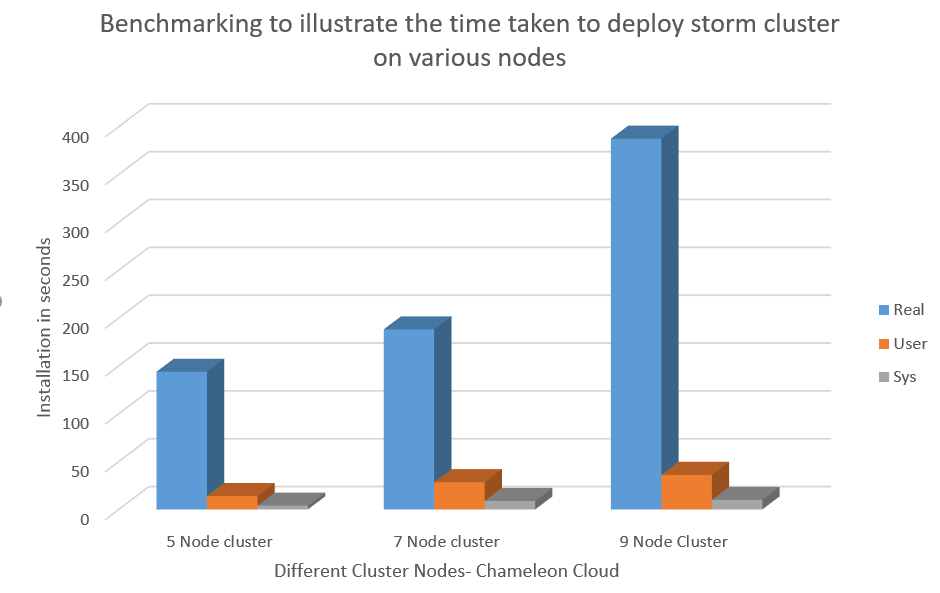
\includegraphics[width=8cm,height=8cm,keepaspectratio,width=\linewidth]{images/bar-1.png}
  \caption{Bar diagram to compare the time taken to deploy on Chameleon}
  \label{barc}
\end{figure}

\subsection{JetStream Cloud}
Automated deployment on Jestream cloud of various cluster node sizes of 5, 7 and 
9 and results are presented as follows, in the form of a table \ref{T:timejet} and 
illustrated as a figure \ref{i:barjet}.

\begin{table}[!htb]
\centering
\caption{Illustrating the various times it took to deploy on Jetstream}\label{T:timejet}
 \begin{tabular}{|c|| c c c|} 
 \hline
 Install Time &  5 node cluster & 7 node cluster & 9 node cluster\\ [0.5ex]
 \hline\hline
 Real: &153.73 &232.923 & 256.675 \\ 
 \hline
 User: & 24.232 & 38.14 & 46.208 \\
 \hline
 Sys: & 5.988 &11.54 & 13.568  \\
 \hline
\end{tabular}
\end{table}

A bar description of the time taken for deployment on different size 
clusters see Fig \ref{i:barjet}.

\begin{figure}[!htb]
  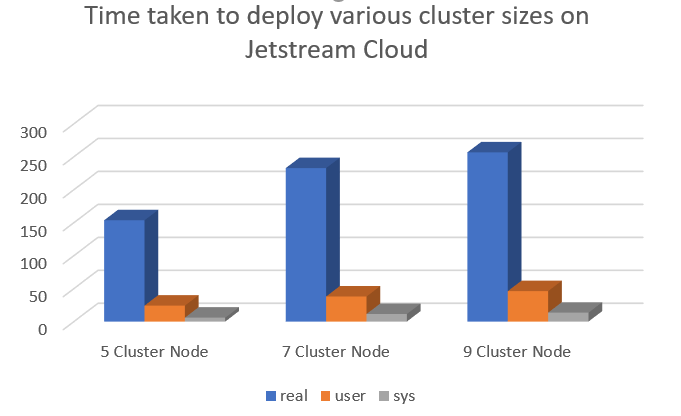
\includegraphics[width=8cm,height=8cm,keepaspectratio,width=\linewidth]{images/bar-2.png}
  \caption{Bar diagram to compare the time taken to deploy on Jetstream }
  \label{i:barjet}
\end{figure}

\subsection{Kilo Cloud - FutureSystems}
Automated deployment on Kilo cloud of various cluster node sizes
of 5, 7 and 9 and results are presented, in the form of a table
\ref{T:timekilo} and illustrated as a figure \ref{i:timekilo}

\begin{table}[!htb]
\centering
\caption{Illustrating the various times it took to deploy on Kilo}\label{T:timekilo}
\begin{center}
 \begin{tabular}{|c|| c c c|} 
 \hline
 Install Time &  5 node cluster & 7 node cluster & 9 node cluster\\ [0.5ex]
 \hline\hline
 Real: & 478.426 & 592.267 & 798.894 \\ 
 \hline
 User: & 53.728 & 61.104 & 77.388 \\
 \hline
 Sys: & 7.048 & 11.224 & 16.116 \\
 \hline
\end{tabular}
\end{center}
\end{table}

A bar description of the time taken for deployment on different size 
clusters see Fig \ref{i:timekilo}.

\begin{figure}[!htb]
  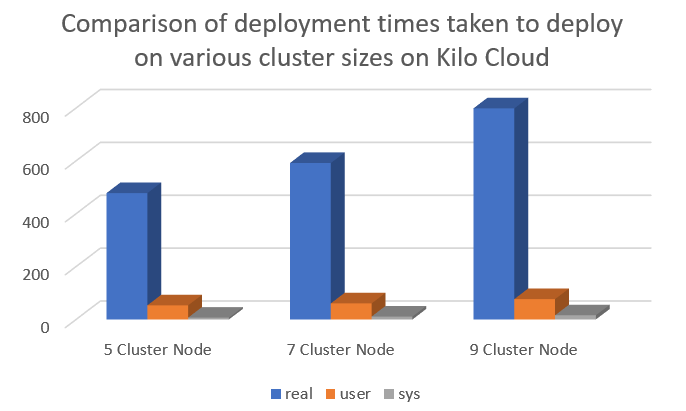
\includegraphics[width=8cm,height=8cm,keepaspectratio,width=\linewidth]{images/bar-3.png}
  \caption{Bar diagram to compare the time taken to deploy on Kilo}
  \label{i:timekilo}
\end{figure}

\section{Deployment Summary on various clouds}
Comparison between installation time on the three clouds with differing
cluster sizes is done in the figure \ref{gvc}. The following inferences 
were made:
\begin{itemize}
\item Kilo cloud - Not conducive to development or production as the
  creation of vms on the cloud and the installation of software took a
  relatively long time.
\item Chameleon and Jetstream clouds have similar rates of
  deployment. As observed, jetstream is more suitable for production.
\item All the clusters took similar amount of time for starting the
  zookeeper and storm processes.
\end{itemize}

The table showcases the times plotted. see Table \ref{T:gvc}
\begin{table}[h]
\begin{center}
  \centering
  \caption{ Time to deploy various cluster sizes on various clouds}
  \label{T:gvc}
 \begin{tabular}{|c|| c c c|} 
 \hline
 Install Time & Chameleon  & Jetstream & Kilo \\ [0.5ex]
 \hline\hline
 5 node: & 161.802 & 183.95 & 539.202\\
 \hline
 7 node: & 305.494 & 282.603 & 664.595 \\
 \hline
 9 node: & 393.716 & 316.451 & 892.398 \\
 \hline
\end{tabular}
\end{center}
\end{table}

A plot has been illustrated to distinguish the installation time on
the different clouds see Fig \ref{gvc}.
\begin{figure}[!htb]
  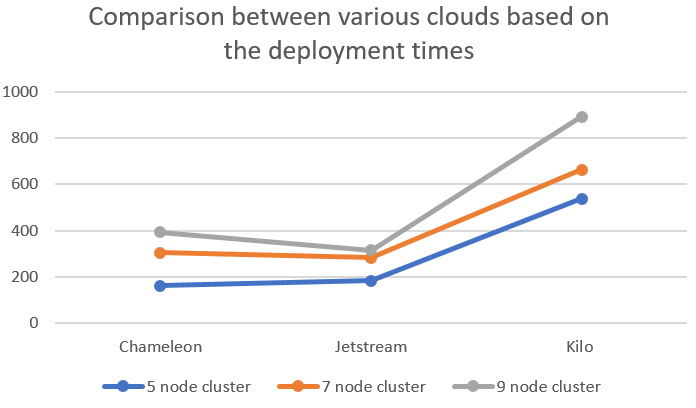
\includegraphics[width=8cm,height=8cm,keepaspectratio,width=\linewidth]{images/bar-4.png}
  \caption{Graph plot to compare the time taken to deploy on various clouds}
  \label{gvc}
\end{figure}

\section{Analysis of Performance Benchmarking on various clouds:}
As a part of this Project we would like to examine the difference in
terms of performance between clouds and analyze the results to discern
the advantages of one cloud over the other. To test the performance, a
topology from the storm-starter project was used. The topology is
based on the basic word count topology with a few changes. The first
difference is the rate of production of sentences. The rate may be set
using arguments. This enable us to perform stress testing on clusters
of different sizes and clouds. The second difference is the number of
worker nodes to be used. This property allows us to accurately define
the number of storm supervisor nodes to run the topology on and gather
the results effectively. The final difference is the time for which
the topology runs. This is an important feature as the metrics are
printed with a period of 30 secs. This implies that every 30s, the
number of sentences that have been executed successfully is printed
and a new set of sentences are generated for the next 30 secs. We have
chosen a value of 5 minutes as this gives us an accurate idea of the
effectiveness of the cluster. The definitions of throughput and
latency are mentioned as follows: \textbf{\textit{Latency}} is the
time required to perform some action or produce a result.
\textbf{\textit{Throughput}} is the number of such actions performed
per unit of time.

A result is produced/completed on a storm cluster when an "ack" is
received. The number of such acks defines the throughput of the
cluster. For example, if we have received 12,600 acks during a 30s
time period, then the throughput rate is 420/sec. Higher throughput
rates are desired for better computing capability with lower latency.


Analysis for the entire cloud based on the mentioned parameters and
tests were performed, the strategy has been done by writing a shell
script, performance.sh which runs for different input sizes for a
given cluster and collects the output in a file. This test has been
performed on all clusters in a given cloud, repeated on different
clouds. All the results are tabulated in the next sections, a detailed
analysis based on the results obtained is also elucidated clearly.



\subsection{Hardware:}
All the nodes on each of the clouds deployed had the following features in 
common:
\begin{description}
\item Image: Ubuntu-14.04-64
\item Flavor: m1.small
\item Nodes: Depending on the cluster size various node sizes are deployed
\end{description}

\subsection{Experimental Results and Analysis:}
Following were the inferences and conclusions derived from the performance
benchmarking, with respect to the ThroughputVsLatency topology.
\begin{itemize}
\item 5 node cluster: The throughput graph starts small and rises
  equally upto a rate of 150000, at which point, the throughput on
  chameleon cloud falls rapidly.  The results on kilo cloud indicate
  that a 5 node cluster is sub-optimal for this cloud. Jetstream cloud
  scaled very well with increase in throughput. The results are
  tabulated here see Table \ref{T:bench-5} and illustrated here see
  Fig \ref{5c}.
\item 7 node cluster: Chameleon cloud performed better on a 7 node
  cluster but the throughput falls rapidly after 300000. Kilo cloud
  performed sub-optimally at all throughput levels. Jetstream cloud
  scaled exceptionally well with an increase in throughput. The
  results are tabulated here see Table \ref{T:bench-7} and illustrated here
  see Fig \ref{7c}.
\item 9 node cluster: The difference in performance between chameleon
  cloud and jetstream cloud is negligible. Kilo cloud performs well
  upto a throughout value of 150000 and falls afterwards. Jetstream
  cloud is consistent at all throughput levels and chameleon cloud
  performed equally well. The results are tabulated here
  see Table \ref{T:bench-9} and illustrated here see Fig \ref{9c}
\item While significant improvements were observed on clusters of
  larger sizes, the results are not consistent at all times for
  chameleon cloud. Jetstream cloud provided consistent results and can
  be used for production clusters as shown by its performance
  results. Kilo cloud is not suitable for deployment or for
  production. The results are consolidated in the form of a graph
  see Fig \ref{ac}.
\end{itemize}

\begin{table}[!htb]
\centering
\caption{Throughput vs Latency on all 5 node clusters on 3 clouds:}\label{T:bench-5}
\begin{center}
 \begin{tabular}{|c|| c c c|} 
 \hline
  &   &5 node cluster & \\ [0.5ex]
 \hline\hline
 Throughput: & Chameleon & Jetstream & Kilo \\ 
 \hline
 3000: & 2940 & 2760 & 2906 \\
 \hline
 15000: & 13958 & 13654 & 15093 \\
 \hline
 30000: & 27946 & 28178 & 30095 \\
 \hline
 150000: & 140454& 142084 &137352 \\
 \hline
 300000: & 35417.5 & 275074 & 10506 \\
 \hline
 450000: & 14946.667 & 414982 & 6268 \\
 \hline
\end{tabular}
\end{center}
\end{table}

\begin{table}[!htb]
\centering
\caption{Throughput vs Latency on all 7 node clusters on 3 clouds:}\label{T:bench-7}
\begin{center}
 \begin{tabular}{|c|| c c c|} 
 \hline
  &   &7 node cluster & \\ [0.5ex]
 \hline\hline
 Throughput: & Chameleon & Jetstream & Kilo \\ 
 \hline
 3000: & 2702 & 2734 & 2875 \\
 \hline
 15000: & 13502 & 13766 & 14348 \\
 \hline
 30000: & 27364 & 28110 & 29160 \\
 \hline
 150000: & 140124& 141894 &41275 \\
 \hline
 300000: & 280170 & 284356 & 431.25\\
 \hline
 450000: & 67857.5 & 412488 & 435 \\
 \hline
\end{tabular}
\end{center}
\end{table}


\begin{table}[!htb]
\centering
\caption{Throughput vs Latency on all 9 node clusters on 3 clouds:}\label{T:bench-9}
\begin{center}
 \begin{tabular}{|c|| c c c|} 
 \hline
  &   &9 node cluster & \\ [0.5ex]
 \hline\hline
 Throughput: & Chameleon & Jetstream & Kilo \\ 
 \hline
 3000: & 2700 & 2754 & 2848 \\
 \hline
 15000: & 14722.22 & 13784 & 14337 \\
 \hline
 30000: & 27724 & 27282 & 29455 \\
 \hline
 150000: & 151562.22& 141580 & 149440 \\
 \hline
 300000: & 305566.667 &286708 & 8832 \\
 \hline
 450000: & 418002 & 427174 & 7312 \\
 \hline
\end{tabular}
\end{center}
\end{table}

\begin{figure}[!htb]
  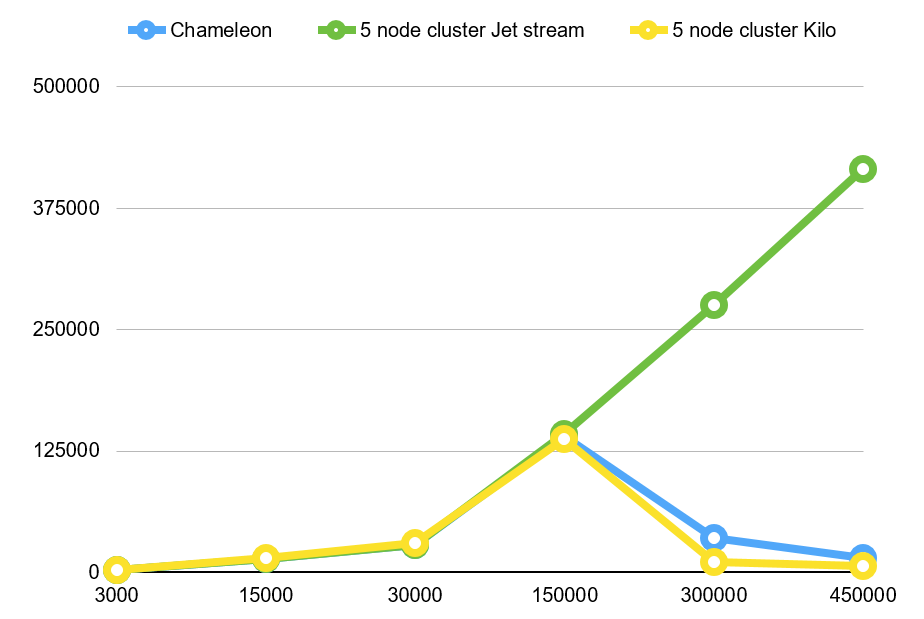
\includegraphics[width=8cm,height=8cm,keepaspectratio,width=\linewidth]{images/bench2-1.PNG}
  \caption{Graph plot to compare the peformance on 5 nodes across various clouds}
  \label{5c}
\end{figure}

\begin{figure}[!htb]
  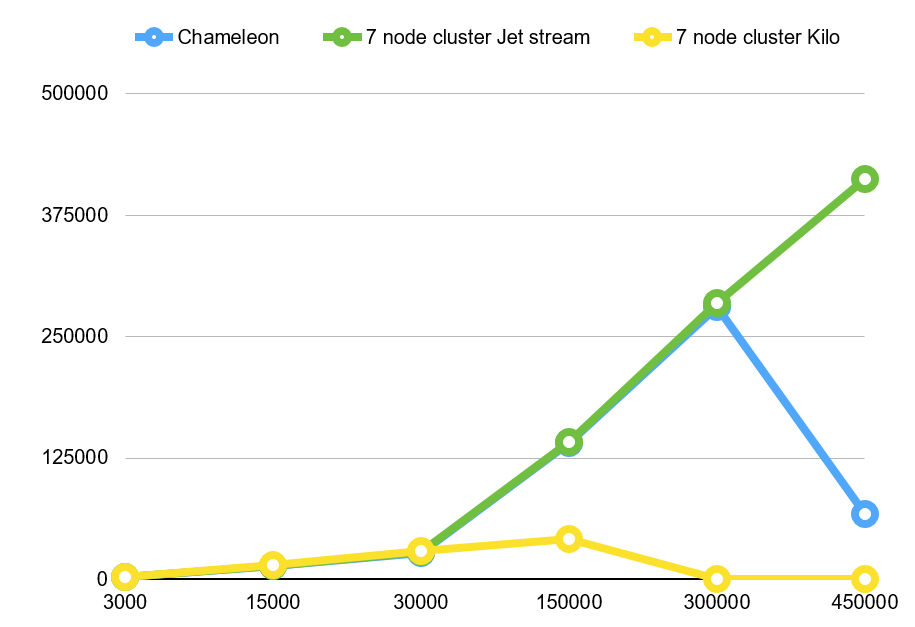
\includegraphics[width=8cm,height=8cm,keepaspectratio,width=\linewidth]{images/bench2-2.PNG}
  \caption{Graph plot to compare the performance on 7 nodes across various clouds}
  \label{7c}
\end{figure}

\begin{figure}[!htb]
  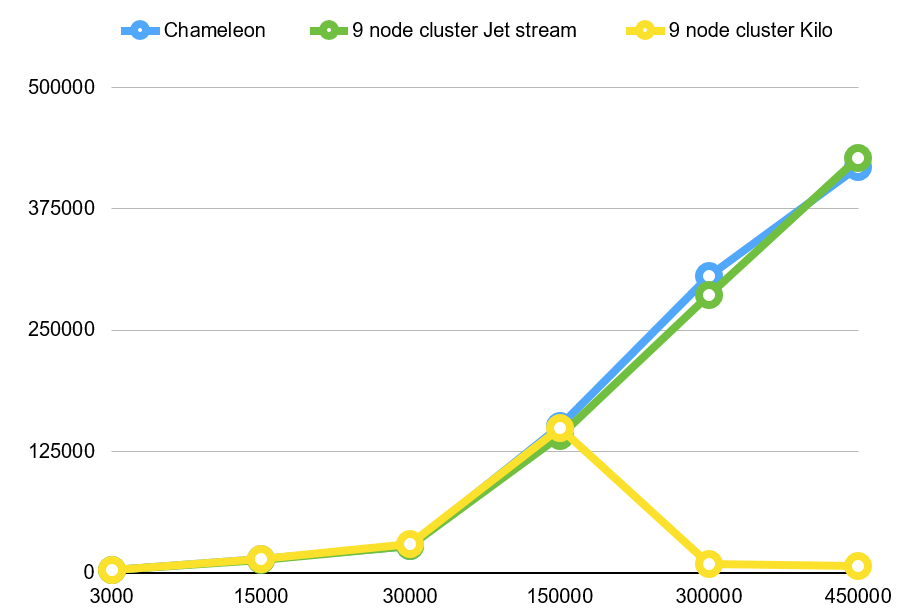
\includegraphics[width=8cm,height=8cm,keepaspectratio,width=\linewidth]{images/bench2-3.PNG}
  \caption{Graph plot to compare the performance on 9 nodes across various clouds}
  \label{9c}
\end{figure}

\begin{figure}[!htb]
  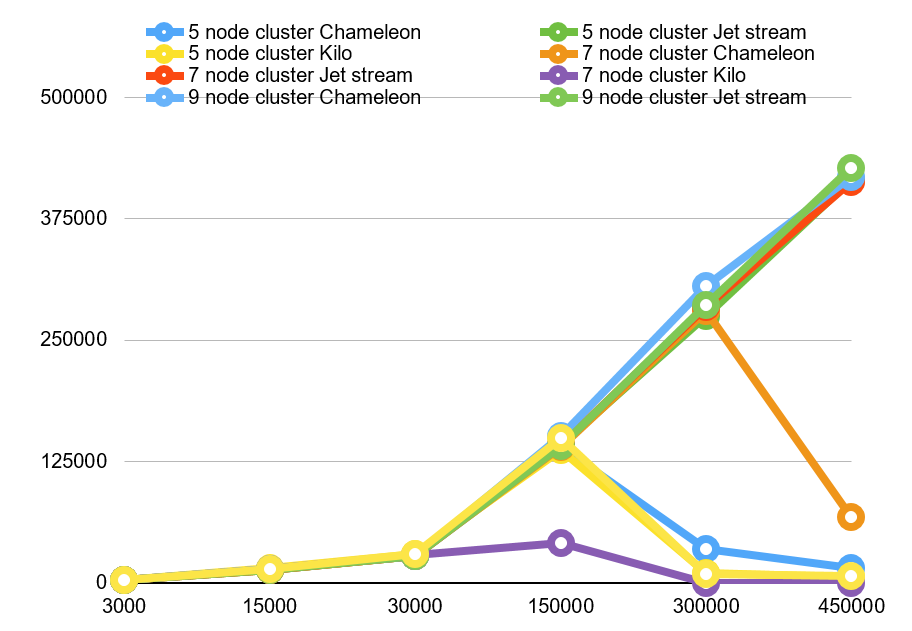
\includegraphics[width=8cm,height=8cm,keepaspectratio,width=\linewidth]{images/bench2-4.PNG}
  \caption{Graph plot to compare the performance on all the nodes across various clouds}
  \label{ac}
\end{figure}

\section{Summary}
We have created, tested and demonstrated a fully automated method to
configure and deploy a Storm cluster which can be deployed on any
cloud environment using cloudmesh. We have deployed it on
Chameleon, Jetstream and Kilo cloud. Benchmarking strategy is envisioned
by viewing the time it takes to deploy a particular cluster on various
cloud environments. We did a benchmark test on Chameleon, Jetstream
and Kilo cloud to measure the time taken to deploy 5, 7 and 9 node
clusters, so far it has shown satisfactory results and we are striving
to take it beyond to other cloud environments as well, outside the
cloudmesh usage. A performance benchmarking has also been done to
better analyze the various cloud performances on deployment of a storm
cluster. We have measured the Throughput and Latency for different
lengths of input to check the performance on various clouds. All the
results have been illustrated and various conclusions drawn based on
the data obtained from the complete deployment of the storm cluster.

\section{Acknowledgments}
This project was a part of the Big Data Software and Projects
(INFO-I524) course. We would like to thank Professor Gregor von
Laszewski and the associate instructors for their help and support
during the course. Special mention to cloudmesh client which made most
of the gruelling taks straighforward.

\section{Code References}
Following were the code resources used in deploying the cluster at various
stages.
\begin{itemize}
\item
  While coding configurations related to Storm we used the following
  resources, we have looked at the sample use cases of the storm
  application at Twitter and Spotify. Code resources for
  Storm-\cite{www-storm1}\cite{www-storm2}\cite{www-storm3}\cite{www-storm4}\cite{www-storm5}\cite{www-storm6}\cite{www-storm7}\cite{www-storm8}\cite{www-storm9}\cite{www-storm10}
\item
 While configuring the Zookeeper cluster, we came across many
 solutions, the important question we came across is whether to use a
 stand-alone mode or a server mode configuration also while
 researching for various cluster sizes, we have come to the conclusion
 that storm is better deployed on cluster sizes more than 5. However,
 the server mode configuration is quite relevant to our project, so
 used many resources for coding the required
 configurations. Zookeeper-\cite{www-zk1}\cite{www-zk2}\cite{www-zk3}\cite{www-zk4}\cite{www-zk5}\cite{www-zk6}\cite{www-zk7}\cite{www-zk8}
\item The following code resources were used in analyzing the
  toplogies which were created part of development of the storm
  cluster. We went through many use-cases such as like in the case of
  Spotify while researching this topic. Running Topologies on a
  cluster-\cite{www-rtc1}\cite{www-rtc2}\cite{www-rtc3}\cite{www-rtc4}\cite{www-rtc5}\cite{www-rtc6}
\item While encountering various issues with Zookeeper, following code
  resources were used, of these we examined whether dynamic toplogies
  where possible to create, problems with running a 3 node cluster,
  and other config files configuration. Zookeeper
  Troubleshooting-\cite{www-zt1}\cite{www-zt2}\cite{www-zt3}\cite{www-zt4}\cite{www-zt5}\cite{www-zt6}
\item While checking the log files to check if storm is working or
  not, had to explore many resources to make sure it was up and
  running. Storm
  Troubleshooting-\cite{www-nnf1}\cite{www-nnf2}\cite{www-nnf3}\cite{www-nnf4}
\item Storm yaml defaults file details were obtained from the many
  code resources.-\cite{www-sd1}
\end{itemize}

\bibliography{references}
\clearpage
\appendix

\section{Work Breakdown}
\begin{itemize}
\item Ajit Balaga: Responsible for deployment of storm cluster on
  various clouds and clusters of different sizes, played an
  instrumental role in understanding the storm and its
  architecture. Developed the cmd5 storm commands extension and
  ansible scripts for deployment, responsible for perfomance
  benchmarking on chameleon cloud, jetstream and 9 node cluster on
  kilo cloud.
\item Vasanth Methkupalli: Responsible for deployment of the storm
  cluster on various clouds of different cluster sizes using ansible,
  almost automated the entire deployment of storm cluster on
  cloud. Performed deployment benchmarking on various clouds and
  analysis. Also, responsible for performance benchmarking on Kilo
  cloud and analysis of the entire Performance bencmarking.
\end{itemize}

\listoffigures
\listoftables
\end{document}
